\documentclass{beamer}
%\usefonttheme{serif}
\usepackage{listings}
\usepackage{pst-solides3d}
\usepackage[lined,boxed]{algorithm2e}
\usepackage{gnuplottex}
\usepackage{texdraw}
\usepackage{graphicx}



%\usepackage{epcc}
\usepackage{graphics}
\usepackage{epigraph}
\usepackage{amsmath}
\usepackage{url}
\usepackage{listings}
\usepackage[binary-units=true]{siunitx}
\usepackage[justification=centering, labelfont=bf, font={small}]{caption}
\usepackage{float}
\usepackage{subcaption}
\usepackage{graphicx}
%\usepackage[margin=3cm]{geometry}
%\usepackage{pst-solides3d}
%\usepackage{texdraw}
%\usepackage{gnuplottex}
%\usepackage{csvsimple}
%\usepackage[lined,boxed]{algorithm2e}
%\usepackage[nottoc]{tocbibind}


\setbeamertemplate{bibliography item}{}

%\setbeamerfont{title}{family=\rm\addfontfeatures{Scale=1.18, Numbers={Lining, Proportional}}}

\title[acoustics] % (optional, only for long titles)
{Modelling Room Acoustics on a GPU}
\subtitle{A new method that improves memory efficiency}
\author[Author] % (optional, for multiple authors)
{Jacob Josiah Webber}
\date[22 August 2017] % (optional)
{Dissertation Presentation}
\subject{HPC}


\begin{document}
\frame{\titlepage}

\begin{frame}
	\frametitle{Introduction}
	This talk aims to answer the following questions:
	\begin{itemize}
		\item Modelling acoustics: what and why?
		\item What is the current state-of-the-art?
		\item What is the new method proposed here?
		\item What were the results when this method was used?
		\item How could these be improved?
	\end{itemize}
\end{frame}



\begin{frame}
	\frametitle{Sound}
	\framesubtitle{What is it?}
	\begin{block}{From Wikipedia}
		``In physics, sound is a vibration that propagates as a typically audible mechanical wave of pressure and displacement, through a transmission medium such as air or water.''
	\end{block}
	\begin{block}{From my undergraduate degree}
		\begin{equation}
			\nabla^{2} P - \frac{1}{{c^2 }}\frac{{\partial ^2 P}}{{\partial t^2 }} = 0
		\end{equation}
	\end{block}
\end{frame}
  
  
\begin{frame}
	\frametitle{Room acoustics}
	\begin{itemize}
		\item The physical properties of rooms affects how we hear sound.
		\item Sound reverberates off walls/objects.
		\item Waves diffract around corners.
		\item Some rooms echo, some sound dry.
		\item Backwards: If we know physical properties can we derive the sound?
	\end{itemize}
\end{frame}
  
  
\begin{frame}
	\frametitle{The wave equation}
	$$\frac{\partial ^2 P}{\partial x^2 } - \frac{1}{{c^2 }}\frac{{\partial ^2 P}}{{\partial t^2 }} = 0$$
	where $P$ is pressure deviation and $c$ is speed of sound in medium.
	\linebreak
	\begin{itemize}
		\item Very familiar to those who have studied physics
		\item It, and its application to acoustics, are derivable from first principles.
		\item Solving for $P$ gives us acoustic properties of a system (boundary conditions are very important!).
		\item Solving this analytically for complex systems is not possible.
	\end{itemize}    
\end{frame}

\begin{frame}
	\frametitle{FTDT}
	\framesubtitle{Finite-difference time-domain method}
	Finite difference methods are a way of approximating and discretising differential equations so that they can be solved numerically.
	\linebreak
	
	Start off by replacing derivative with finite difference:
	
	%Effectively turns solving differential equation into a large stencilling operation.
	
	
	\begin{equation}
		\label{equation:difference}
		\frac{df(u)}{du} \approx \frac{f(u+h) - f(u-h)}{2h}
	\end{equation}
	
	\begin{equation}
		\label{equation:difference-second}
		\frac{d^{2}f(u)}{du^{2}} \approx \frac{f(u+h) - 2f(u) + f(u-h)}{h^{2}}
	\end{equation}
\end{frame}


\begin{frame}
	Let $h$ be the distance between samples ($H$) and $P$ be a 3D grid
	\begin{equation}
		\label{equation:part1}
		\delta_{t}^{2} P_{l,m,p}^{n} \equiv \frac{1}{T^{2}} \Big(P_{l,m,p}^{n+1} - 2 P_{l,m,p}^{n} + P_{l,m,p}^{n-1}\Big) \approx \frac{{\partial ^2 P}}{{\partial t^2 }}
	\end{equation}
	
	\begin{equation}
		\label{equation:part2}
		\delta_{x}^{2} P_{l,m,p}^{n} \equiv \frac{1}{H^{2}} \Big(P_{l+1,m,p}^{n} - 2 P_{l,m,p}^{n} + P_{l-1,m,p}^{n}\Big) \approx \frac{{\partial ^2 P}}{{\partial x^2 }}
	\end{equation}
	
	\begin{equation}
		\label{equation:part3}
		\delta_{y}^{2} P_{l,m,p}^{n} \equiv \frac{1}{H^{2}} \Big(P_{l,m+1,p}^{n} - 2 P_{l,m,p}^{n} + P_{l,m-1,p}^{n}\Big) \approx \frac{{\partial ^2 P}}{{\partial y^2 }}
	\end{equation}
	
	\begin{equation}
		\label{equation:part4}
		\delta_{z}^{2} P_{l,m,p}^{n} \equiv \frac{1}{H^{2}} \Big(P_{l,m,p+1}^{n} - 2 P_{l,m,p}^{n} + P_{l,m,p-1}^{n}\Big) \approx \frac{{\partial ^2 P}}{{\partial z^2 }}
	\end{equation}
\end{frame}


\begin{frame}

Taking the expanded 3D wave equation
	\begin{equation}
		\label{equation:wave-expanded}
		\frac{{\partial ^2 P}}{{\partial t^2 }} = c^2 \Bigg( \frac{\partial ^2 P}{\partial x^2 } + \frac{\partial ^2 P}{\partial y^2 }  + \frac{\partial ^2 P}{\partial z^2 } \Bigg)
	\end{equation}
	This can be replaced with finite differences:
	\small
	\begin{multline}
		\label{equation:stencil-big}
		P_{l,m,p}^{n+1} - 2 P_{l,m,p}^{n} + P_{l,m,p}^{n-1} = \frac{c^2 T^2}{H^2} \big(P_{l+1,m,p}^{n} + P_{l-1,m,p}^{n} + P_{l,m+1,p}^{n} + P_{l,m-1,p}^{n} \\ 
		+ P_{l,m,p+1}^{n} + P_{l,m,p-1}^{n} - 6 P_{l,m,p}^{n} \big)
	\end{multline}
\end{frame}

\begin{frame}
	Letting the Courant number be defined as 
	
	\begin{equation}
		\lambda \equiv \frac{c T}{H}
	\end{equation}
	
	and our stencil 
	
	\begin{equation}
		\label{equation:s-define}
		S \equiv P_{l+1,m,p}^{n} + P_{l-1,m,p}^{n} + P_{l,m+1,p}^{n} + P_{l,m-1,p}^{n} + P_{l,m,p+1}^{n} + P_{l,m,p-1}^{n}
	\end{equation}
	
	gives a somewhat neater version of equation \ref{equation:stencil-big}
	
	\begin{equation}
		\label{equation:stencil-small}
		P_{l,m,p}^{n+1} = (2 - 6 \lambda^2)P_{l,m,p}^{n} + \lambda^2 S - P_{l,m,p}^{n-1}
	\end{equation}
\end{frame}

\begin{frame}
	\frametitle{Stencil}
	\begin{figure}
		\centering
		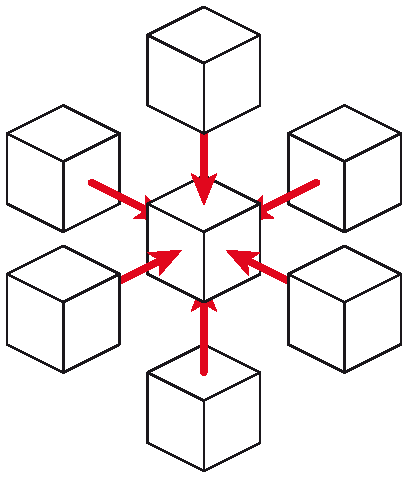
\includegraphics[width=0.5\textwidth]{../diagrams/stencil}
		\label{stencil}
	\end{figure}
\end{frame}


\begin{frame}
	\frametitle{Memory considerations}
	For stencilling operations, memory access is the bottleneck.
	\begin{itemize}
		\item Accurate models need a lot of points to model a room.
		\item Wavelength of sound at 20kHz is 17mm.
		\item High memory bandwidth means GPUs are used - limited memory.
		\item Standard 3d arrays are cuboid.
		\item Due to memory layout, neighbouring points in space will always be far apart in memory.
	\end{itemize}
\end{frame}
 
\begin{frame}
	\begin{figure}
		\centering
		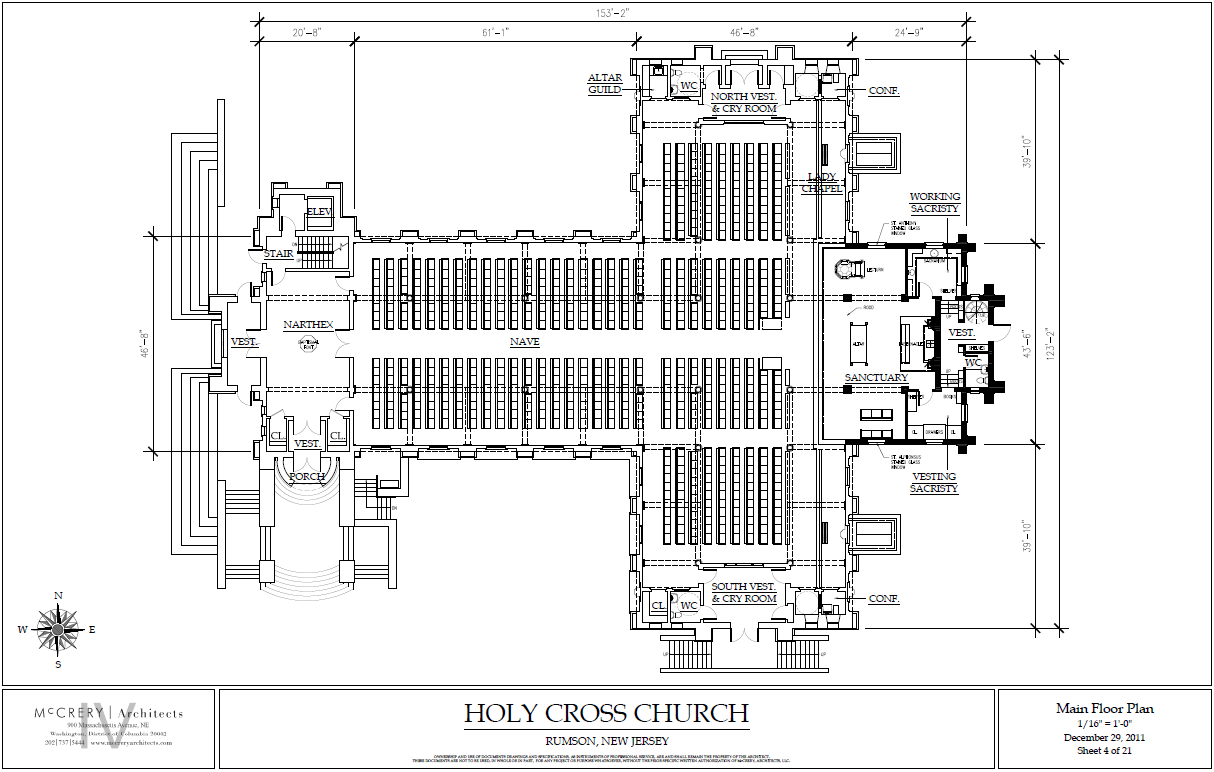
\includegraphics[width=\textwidth]{../diagrams/church}
		\label{church}
	\end{figure}
\end{frame}

\begin{frame}
\frametitle{The \emph{Bounding Box}}
\framesubtitle{The current method with irregularly shaped rooms}
	\begin{itemize}
		\item An array of $K$ values encodes the shape of the room.
		\item These are required to perform stencil with boundary conditions.
		\item Requires another array to be stored - can be chars.
		\item Store and operate on points that are outside the room - waste!
	\end{itemize}
	Stencil operation with these values becomes:
	\begin{equation}
\label{equation:stencil-boundary}
P_{l,m,p}^{n+1} = (2 - \lambda^2 K_{l,m,p} )P_{l,m,p}^{n} + \lambda^2 S - P_{l,m,p}^{n-1}
\end{equation}
(Actual stencil is a bit more complicated and includes a wall permittivity term)
\end{frame}



\begin{frame}
\frametitle{The \emph{Bounding Box}}
\framesubtitle{The current method with irregularly shaped rooms}
Each CUDA kernel is allocated a block of the room the same size as its block of threads.
Many of these blocks will be completely outside the room!
\IncMargin{1em}
\begin{algorithm}[H]
\footnotesize
 \KwData{Three dimensional arrays of $P_{l,m,p}^{n}$, $P_{l,m,p}^{n-1}$ and $K_{l,m,p}$}
 \KwResult{Updated array of $P_{l,m,p}^{n+1}$}
 Get the 3D indices of the current thread from the block and thread IDs\;
 \If{$K_{l,m,p}$ is not zero}{
 	Compute the linear address from the 3D indices\;
 	Overwrite node $P_{l,m,p}^{n-1}$ with $P_{l,m,p}^{n+1}$\;
 }
 Swap pointers.
 \caption{CUDA kernel for update on an irregularly shaped room.}
\end{algorithm}
\end{frame}


\begin{frame}
	\frametitle{The Proposal}
	Use an array of structs instead!
	\begin{itemize}
		\item Store enough points for CUDA kernel to operate on.
		\item Only store structs with at least one point inside the room.
		\item Experiment with different sized arrays within the struct to see if caching benefits can be yielded.
	\end{itemize}
\end{frame}  
  
\begin{frame}[fragile]
	\frametitle{The Struct}
	
	\begin{lstlisting}[caption=The block struct]
typedef real bl_array[Bz][By][Bx];
struct block {
    int up;
    int down;
    int left;
    int right;
    int fore;
    int aft;
    bl_array u;
    bl_array u1;
    char k[Bz][By][Bx];
};
\end{lstlisting}
\end{frame}

\begin{frame}
	\frametitle{Converting between representations}
	\framesubtitle{Going from bounding box to array of structs}
	\IncMargin{1em}

\begin{algorithm}[H]
%\fontsize{6pt}{\linewidth}
  \scriptsize
\label{alg:bound-ss}
 \KwData{Three dimensional array of $K_{l,m,p}$ for a given room}
 \KwResult{Array of blocks (AOB), block locations, number of internal blocks ($T_{i}$)}
 Divide $K_{l,m,p}$ into Bx by By by Bz sized blocks\;
 \While{not at end of blocks}{
  do nothing\;
  \eIf{block contains non-zero $K_{l,m,p}$ value}{
   increment $T_{i}$\;
   store block's location\;
   }{
   	store zero as block location
   }
   go to next block\;
 }
 allocate memory for $T_{i}$ block structs\;
 \While{not at end of block locations}{
 	\If{block location has non-zero value}{
 		copy $K_{l,m,p}$ values to correct block in AOB\;
 	}
 	go to next block location\;
 }
 \caption{Convert bounding box to array of blocks}
\end{algorithm}
\end{frame}

\begin{frame}
\frametitle{Results}
Two things are important:
\begin{itemize}
\item Memory capacity performance.
\item Stencil performance.
\end{itemize}

Tests were run on three different shaped rooms.
\end{frame}

\begin{frame}
\frametitle{But first: Correctness}
For conversion algorithm: wrote a function that converts from bounding box coordinates to block index and array indices within block. Then loop through whole room to check $K$ values. All good!
\linebreak

For stencil: Compare with Matlab script from AAG that implements bounding box method. All good!
\linebreak

To do: compare with real room or analytical solution to simple room.
\end{frame}

\begin{frame}
\frametitle{Memory Capacity Results}
\framesubtitle{Sphere}

\begin{figure}[H]
\centering

\resizebox{0.5\linewidth}{0.25\linewidth}{\begin{pspicture}[shift=*](-4.2,-4.2)(4.2,4.2)

\psset{lightsrc=10 20 30,viewpoint=30 10 30 rtp2xyz,Decran=40}

 %\axesIIID(3,3,3)(6,4,4)
%\psgrid
\psSolid[
object=sphere,
r=2,
ngrid=18 18, axesboxed]%

\psSolid[
action=draw,
object=cube,
RotZ=30,
%show=all,
]%

\end{pspicture}}
\caption{Computer graphic showing a sphere of unit diameter within a cube of unit side.}
\label{figure:sphere-cube}
\end{figure}

\end{frame}









\begin{frame}[fragile]
\begin{figure}[H]
%\centering%
\begin{gnuplot}[terminal=epslatex, terminaloptions=color dashed]
set xlabel "Diameter (Grid Points)"
set autoscale
set ylabel "$\\frac{S_{ss}}{S_{s}}$"
#set style data linespoints
set size 0.8,0.8

plot "../../semi-structured/results/data/memory-cap_graph" \
with lines lt 1 lc rgb "blue" notitle, \
"../../semi-structured/results/data/memory-cap_graph" \
lc rgb "blue" notitle, \
pi/6 lt 2 lc rgb "red" notitle
\end{gnuplot}
\caption{The fraction of memory used by the semi-structured approach with respect to the structured approach (double precision). The ideal fraction of $\frac{\pi}{6}$ is shown as a dashed line}%

\label{figure:cap-sphere}%
\end{figure}%

\end{frame}



\begin{frame}
\frametitle{Memory Capacity Results}
\framesubtitle{Cube}
\begin{itemize}
\item Forms the worst case scenario for AOS method.
\item Integer indices of neighbouring blocks are extra overhead.
\item This overhead is
\end{itemize}

Single Precision:
\begin{equation}
\frac{S_{ss}}{S_{s}} = 1 + \frac{24}{9\cdot\lstinline|Bx|\cdot\lstinline|By|\cdot\lstinline|Bz|}
\label{equation:single-neghbours}
\end{equation}

Double Precision:
\begin{equation}
\frac{S_{ss}}{S_{s}} = 1 + \frac{24}{17\cdot\lstinline|Bx|\cdot\lstinline|By|\cdot\lstinline|Bz|}
\label{equation:double-neghbours}
\end{equation}
\end{frame}

\begin{frame}
\frametitle{Memory Capacity Results}
\framesubtitle{Cube}
\begin{itemize}
\item Sub-arrays of size 8 x 8 x 8
\item Yields $\frac{S_{ss}}{S_{s}} = 1.002757$
\item This matches experimental results for cube for all sizes of room tested.
\end{itemize}
\end{frame}

\begin{frame}[fragile]
\frametitle{Memory Capacity Results}
\framesubtitle{cross}
\begin{figure}[H]
\centering
\resizebox{0.5\linewidth}{0.25\linewidth}{\begin{pspicture}[shift=*](-4.2,-4.2)(4.2,4.2)
%
\psset{lightsrc=10 20 30,viewpoint=30 10 30 rtp2xyz,Decran=40,unit=1}

 %\axesIIID(3,3,3)(6,4,4)
%\psgrid
%\psgrid
\psSolid[
action=draw**,
object=cube,
a=2,
RotZ=00,
%show=all,
](0,-2,0)
\psSolid[
action=draw**,
object=cube,
a=2,
RotZ=00,
%show=all,
](-2,0,0)
\psSolid[
action=draw**,
object=cube,
a=2,
RotZ=00,
%show=all,
](0,0,0)
\psSolid[
action=draw**,
object=cube,
a=2,
RotZ=00,
%show=all,
](2,0,0)



\psSolid[
action=draw**,
object=cube,
a=2,
RotZ=00,
%show=all,
](0,2,0)
%show=all,
%

\end{pspicture}}
\caption{A cross made up of 5 equal cubes.}
\label{figure:cross}
\end{figure}
\end{frame}

\begin{frame}
\frametitle{Memory Capacity Results}
\framesubtitle{cross}
\begin{itemize}
\item Bounding box would take 9 cubes.
\item Cross takes 5 cubes.
\item Ideal bounding box performance would take $\frac{5}{9}\cdot1.002757$
\item This was achieved performance in all cases tested.
\item $\frac{S_{ss}}{S_{s}} = 0.557087$
\end{itemize}
\end{frame}

\begin{frame}
\frametitle{Memory Capacity Results}
\framesubtitle{Quantifying}
\emph{Ideal} is taken to be where two floating point numbers and one char is stored per grid point.
\begin{table}[h!]
\centering
\scriptsize
 \begin{tabular}{|c|c|c|c|c|c|} \hline
 Room Shape & Diam & Ideal (\SI{}{\mebi\byte}) & \multicolumn{2}{c|}{Achieved minus Ideal (\SI{}{\mebi\byte})} & Improvement \\ \cline{4-5}
  &  &  & Structured & Semi-structured & \\ \hline

Cube & 768 & 7344 & 0 &  20.25 & N/A \\
Sphere & 768 & 3845 & 3499 & 168.7 & 20.7X \\  
Cross & 488 & 9221 & 7736 & 226.4 & 34.2X \\  \hline
\end{tabular}
\caption{Quantifying the memory capacity improvements by comparing unecessary data stored between both methods.}
\label{table:cap-quant}
\end{table}
\end{frame}

\begin{frame}
\frametitle{Stencil Performance}

No point in optimising for less memory if the result is slower than CPU code!
\begin{table}[h!]
\centering
\tiny
 \begin{tabular}{|c|c|c|c|c|c|c|} \hline
 Room Shape & Diam & \multicolumn{2}{c|}{Memory Use (MiB)} & \multicolumn{2}{c|}{Time (s)} & Speed-up \\ \cline{3-6}
  &  & Structured & Semi-structured & Structured & Semi-structured & \\ \hline
   
Cube & 608 & 3643.84 & 3653.90 & 79.49 & 81.25 & 0.98X \\  
Sphere & 608 & 3643.84 & 2012.92 &  79.50 & 44.78 & 1.78X \\
Cross & 256 & 2448.00 & 1363.76 & 53.27 & 30.34 & 1.76X \\  \hline
\end{tabular}
\caption{Performance results for the stencilling operation. }
\label{table:perf}
\end{table}
(It's not slower than CPU code)
\end{frame}

\begin{frame}
\frametitle{Stencil Performance}
It's a bit easier to see what's going on when you look at the data processing rates.

\begin{table}[H]
\centering
\small
 \begin{tabular}{|c|c|c|} \hline
 Room Shape & \multicolumn{2}{c|}{Data Rate (\SI{}{\gibi\byte\per\second})} \\ \cline{2-3}
  & Structured & Semi-structured \\ \hline
Cube & 44.77 & 43.92 \\ 
Sphere & 44.76 & 43.90 \\ 
Cross & 44.88 & 43.90 \\  \hline
Mean & 44.80 & 43.91 \\ \hline
\end{tabular}
\caption{Data processing rates.}
\label{table:data}
\end{table}
\end{frame}


\begin{frame}
\frametitle{To Do}
3 months and 1500 lines of CUDA code later there is still plenty to do
\begin{itemize}
\item Check stencil with analytical solution with simple case
\item Compare results with real room
\item Optimize to take advantage of HBM2
\item Port to OpenCL?
\end{itemize}
\end{frame}


\begin{frame}
	\frametitle{The End}
	This talk aimed to answer the following questions:
	\begin{itemize}
		\item Modelling acoustics: what and why?
		\item What is the current state-of-the-art?
		\item What is the new method proposed here?
		\item What were the results when this method was used?
		\item How could these be improved?
	\end{itemize}
\end{frame}

% etc
\end{document}